\section{Sparse autoencoders}
\label{sec:sae}

\begin{sessioncard}
\textbf{Session 5.} \emph{Goal:} understand the tool with which the field currently tries to find the feature
directions of a real model without supervision, and learn to distrust it in the right places.
\emph{Experiments:} a public dictionary for GPT-2 small and how well it reconstructs (\cref{exp:saestats}), what
its latents respond to (\cref{exp:latents}), whether a latent deserves its label (\cref{exp:genderlatents}), and
steering text with one latent (\cref{exp:steertext}).
\emph{Prerequisites:} sessions 3 and 4.
\end{sessioncard}

Session 4 ended with a problem: given many activation vectors, find a large set of directions such that every
vector is a combination of a few of them. Session 3 found one such direction with the help of labels. The
\emph{sparse autoencoder} (SAE) looks for all of them at once and needs no labels. An \emph{autoencoder} is a
network that is trained to reproduce its own input after passing it through an intermediate representation.
Here the intermediate representation is required to be sparse. The method was introduced to interpretability
by \citet{bricken2023monosemanticity} and \citet{cunningham2024sparse}.

\subsection{Definition}

We fix a place in the model, for instance the residual stream at the input of layer 8, and collect its
activation $x\in\R^d$ at every token of a large text collection. An SAE with $m$ \emph{latents}, where $m$ is
much larger than $d$, consists of an encoder and a decoder,
\begin{equation}\label{eq:sae}
\hat f(x) \;=\; \relu\big(\Wenc\,(x-\bdec)+\benc\big)\in\R^m,\qquad
\hat x(x) \;=\; \Wdec\,\hat f(x)+\bdec\in\R^d ,
\end{equation}
with matrices $\Wenc\in\R^{m\times d}$, $\Wdec\in\R^{d\times m}$ and bias vectors $\benc\in\R^m$, $\bdec\in\R^d$.
We write $\Wdec[j]\in\R^d$ for column $j$ of the decoder and call it the \emph{dictionary direction} of latent
$j$. The columns are kept at unit norm. The parameters are trained to minimise
\begin{equation}\label{eq:saeloss}
\text{loss} \;=\; \E\Big[\big\|x-\hat x(x)\big\|^2+\lambda\sum_{j=1}^{m}\hat f_j(x)\Big],\qquad\lambda>0,
\end{equation}
where the expectation is over the collected activations. The first term asks for a faithful reconstruction.
The second term is a penalty on the sum of the latent activations, which are never negative. It pushes most of
them to zero. \Cref{fig:sae} (left) shows the architecture. Note that this is a second, small network that is
trained on the activations of the language model. The language model itself is not changed.

Comparing $\hat x(x)=\bdec+\sum_j\hat f_j(x)\,\Wdec[j]$ with \eqref{eq:lrh}, we see what is hoped for: the
dictionary directions $\Wdec[j]$ should be the feature directions $v_j$, and the latent activations $\hat f_j(x)$
should be the feature activations $f_j$. The hat is a reminder that a latent activation is an estimate. We keep
the two notions apart by name. A \emph{latent} is a unit of an SAE, which we can compute. A \emph{feature} is a
property that the model represents, which we want to know. Whether a given latent corresponds to a feature is an
empirical question in every single case.

\begin{figure}[t]
\centering
\begin{tikzpicture}[>=Latex, font=\small]
\foreach \y/\c in {0/60,1/25,2/80,3/40,4/15} {\draw[tutgrey, fill=tutblue!\c] (0,0.34*\y) rectangle +(0.34,0.34);}
\node[below, align=center] at (0.17,-0.05) {$x\in\R^d$};
\foreach \y in {0,...,12} {\draw[tutgrey, fill=white] (3.1,0.34*\y-1.36) rectangle +(0.34,0.34);}
\draw[tutgrey, fill=tutred!80] (3.1,0.34*3-1.36) rectangle +(0.34,0.34);
\draw[tutgrey, fill=tutred!35] (3.1,0.34*9-1.36) rectangle +(0.34,0.34);
\node[below, align=center] at (3.27,-1.41) {$\hat f(x)\in\R^m$\\ few nonzero};
\foreach \y/\c in {0/55,1/30,2/75,3/40,4/20} {\draw[tutgrey, fill=tutblue!\c] (6.2,0.34*\y) rectangle +(0.34,0.34);}
\node[below, align=center] at (6.37,-0.05) {$\hat x(x)\in\R^d$};
\draw[->, tutgrey] (0.5,0.85) -- node[above] {encoder} (2.95,0.85);
\draw[->, tutgrey] (3.6,0.85) -- node[above] {decoder} (6.05,0.85);
\end{tikzpicture}
\hfill
\begin{tikzpicture}
\begin{axis}[width=6.0cm, height=4.7cm, xmin=0, xmax=1, ymin=0, ymax=1, axis lines=left,
  xlabel={true activation $f$}, ylabel={optimal latent activation $\hat f$}, label style={font=\small},
  tick label style={font=\footnotesize}, xtick={0,0.5,1}, ytick={0,0.5,1}, clip=false]
\addplot[dashed, tutgrey, domain=0:1, samples=2] {x};
\addplot[tutred, very thick, domain=0:1, samples=201] {max(0,x-0.2)};
\node[font=\footnotesize, tutgrey, anchor=south east] at (axis cs:0.74,0.76) {no shrinkage};
\node[font=\footnotesize, tutred!80!black, anchor=north west] at (axis cs:0.62,0.40) {$\max(0,f-\lambda/2)$};
\end{axis}
\end{tikzpicture}
\caption{Left: a sparse autoencoder maps an activation to a much longer vector with few nonzero entries and
back. Right: the latent activation that minimises reconstruction error plus penalty (\cref{prop:shrink}, drawn
for $\lambda=0.4$) lies below the true activation by $\lambda/2$.}
\label{fig:sae}
\end{figure}

\subsection{A dictionary for GPT-2 small}

\begin{experiment}[How good is the reconstruction?]\label{exp:saestats} \script{exp\_sae.py}
We use a public SAE for the residual stream of GPT-2 small at the input of layer 8 \citep{bloom2024open}. It
has $m=24{,}576$ latents for $d=768$ dimensions and was trained with a loss of the form \eqref{eq:saeloss} on
300 million tokens. We evaluate it on $38{,}100$ tokens of other text. The start token of every text is left
out of all statistics and of all interventions of this session, because the stream at this position is very
different from the stream at all others.
\begin{itemize}
\item \textbf{Sparsity.} On average $72$ of the $24{,}576$ latents are active on a token (\cref{fig:saestats},
left). A typical latent fires on about one token in a thousand (right).
\item \textbf{Reconstruction.} The reconstruction $\hat x$ explains $82\%$ of the variance of $x$. This means
that the average of $\|x-\hat x\|^2$ over all tokens is $18\%$ of the average squared distance between $x$ and
the mean activation. Measured from $\bdec$, the reconstruction is on average $0.84$ times as long as $x$.
\item \textbf{Effect on the model.} We run GPT-2 small with $x$ replaced by $\hat x$ at every position. The loss
of the model on the next token rises from $3.55$ to $3.79$. If the stream is replaced by zero instead, the loss
is $11.57$. So the dictionary preserves $97\%$ of what this place of the model contributes to the prediction,
and loses $3\%$.
\item \textbf{Geometry.} The dictionary is close to an instance of \cref{prop:jl}: it consists of $24{,}576$
unit vectors in $768$ dimensions. Among $2000$ of them, the inner products of pairs have a standard deviation of
$0.054$, not much more than the $0.036$ of random vectors, and $99.8\%$ of the pairs are below $0.3$ in absolute
value. The agreement is not complete. Of the pairs, $5.7\%$ exceed $0.1$, against $0.5\%$ for random vectors,
and the largest inner product is $0.85$: some latents have almost the same direction.
\end{itemize}
\end{experiment}

\begin{figure}[t]
\centering
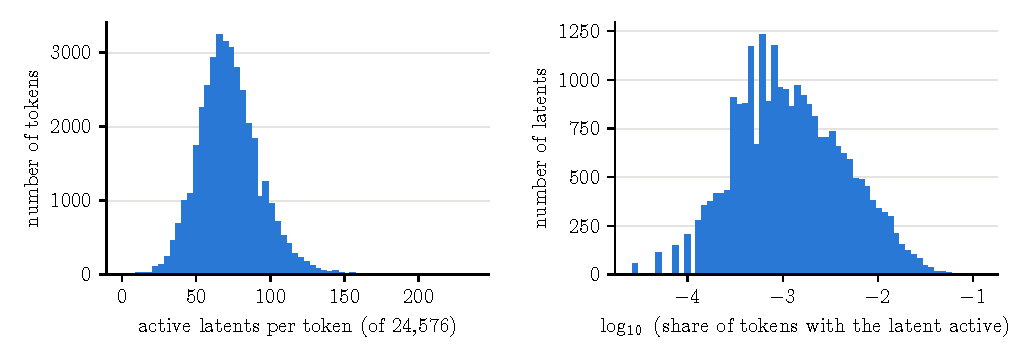
\includegraphics[width=0.95\textwidth]{figures/fig_sae_stats.pdf}
\caption{A public sparse autoencoder with $24{,}576$ latents on the residual stream of GPT-2 small
(\cref{exp:saestats}). Left: number of active latents per token. Right: how often each latent fires.}
\label{fig:saestats}
\end{figure}

No single number says whether a dictionary is good. A dictionary is judged by its reconstruction, its sparsity
and its effect on the model together, and these trade off against one another \citep{karvonen2025saebench}.

\begin{experiment}[What latents respond to]\label{exp:latents} \script{exp\_sae.py}
For a latent we look at two things: the tokens on which it is most active, and the tokens whose logits its
dictionary direction raises most strongly when it is read by the unembedding as in \cref{prop:dla}.
\Cref{tab:latents} shows six latents. They are far easier to read than the neurons of \cref{tab:neurons}, and
they are of different kinds. Latent 5238 fires on the hyphen after \tok{cross} and promotes \tok{sectional},
\tok{border} and \tok{cultural}: it stores what should come next. Latent 614 is about a topic, WikiLeaks,
whichever token expresses it. Latent 1088 is grammatical: it fires on adjectives and promotes the endings that
an adjective can take. The table was selected by us from many candidates, and not every latent is this clean.
In latent 824 the three strongest examples are about livestock, and further down its list there are tokens
that are not.
\end{experiment}

\begin{table}[t]
\centering\small
\begin{tabular}{@{}r>{\raggedright\arraybackslash}p{0.13\textwidth}>{\raggedright\arraybackslash}p{0.39\textwidth}>{\raggedright\arraybackslash}p{0.33\textwidth}@{}}
\toprule
Latent & Our label & Strongest activations (token in brackets) & Tokens it promotes \\
\midrule
5238 & after \tok{cross-} & \tok{population-based cross[-]}, \tok{covalently cross[-]}, \tok{the cross[-]} &
\tok{sectional}, \tok{examination}, \tok{disciplinary}, \tok{border}, \tok{cultural} \\ \addlinespace
614 & WikiLeaks & \tok{government emails[ WikiLeaks]}, \tok{Wiki[Leaks]}, \tok{WikiLeaks[ has]} &
\tok{Leaks}, \tok{founder}, \tok{cables}, \tok{WikiLeaks}, \tok{dumps} \\ \addlinespace
824 & livestock & \tok{looting,[ cattle]}, \tok{scene at a[ poultry]}, \tok{incident at a[ poultry]} &
\tok{grazing}, \tok{herds}, \tok{ranch}, \tok{yards}, \tok{meat} \\ \addlinespace
1088 & adjectives & \tok{finding[ sharp]}, \tok{sing a[ loud]}, \tok{effective and[ precise]} &
\tok{ened}, \tok{ening}, \tok{est}, \tok{ness}, \tok{ener} \\ \addlinespace
658 & first names & \tok{[Justin]}, \tok{[Jake]}, \tok{[Peter]}, \tok{Ben[jamin]}, \tok{[ Henry]} &
\tok{Roberts}, \tok{Matthews}, \tok{Davis}, \tok{Reed}, \tok{Miller} \\ \addlinespace
18206 & female first names & \tok{Kat[ie]}, \tok{And[rea]}, \tok{Jul[ie]}, \tok{Re[becca]}, \tok{M[olly]} &
\tok{Marie}, \tok{Lynn}, \tok{Mae}, \tok{Louise}, \tok{Anne} \\
\bottomrule
\end{tabular}
\caption{Six latents of the sparse autoencoder of \cref{exp:saestats}. The labels are ours
(\cref{exp:latents}).}
\label{tab:latents}
\end{table}

\subsection{Does a latent deserve its label?}

A label that was read off the strongest examples is a hypothesis. We test four latents on the prompts of
session 3, where we know the ground truth: 56 male and 56 female names.

\begin{experiment}[Four candidates for one concept]\label{exp:genderlatents} \script{exp\_sae.py}
We encode the stream at the position of the name, at the input of layer 8, and compare with the difference of
means between female and male names at the same place.
\begin{itemize}
\item \textbf{Latent 18206}, ``female first names'', fires on all 56 female names and on none of the male
names. Its dictionary direction has a cosine of $0.68$ with the difference of means. The label holds.
\item \textbf{Latent 658}, ``first names'', fires on all 112 names, as its label says.
\item \textbf{Latent 13484} looks like a second latent for female names: its strongest examples in our text are
\tok{Mary}, \tok{Molly}, \tok{Lily} and \tok{Carol}. It fires on $11\%$ of the female names. The strongest
examples suggested a general concept, and the latent covers a small part of it.
\item \textbf{Latent 11952} has the dictionary direction that is most aligned with the difference of means, with
a cosine of $0.76$. It fires on one of the 112 names. Its strongest examples are words such as \tok{actress} and
\tok{Daughters}. A direction that points the right way is not the same as a latent that is active.
\end{itemize}
Then we intervene. For the male names, the logit difference $\logit(\tok{she})-\logit(\tok{he})$ is $-3.3$.
Adding the direction of latent 18206 at the name, with the strength that it has on female names, moves it to
$-2.4$. Adding the three latents whose activation differs most between the two groups moves it to $-2.0$.
Random latents with the same strength leave it at $-3.2$, on average over ten latents. Adding the difference of
means moves it to $+0.3$.
\end{experiment}

The experiment shows both sides of the method. Without any labels, the SAE has found a direction that
separates female from male names perfectly and that the model uses, since steering along it shifts the logit
difference by $0.9$ towards \tok{she} and steering along random latents does not. And this latent carries only a quarter of the effect of the
supervised direction. The concept is spread over several latents, and one latent is a part of it. Its
contribution to the stream has norm $9.7$, against $42$ for the difference of means.

\begin{experiment}[Steering text with one latent]\label{exp:steertext} \script{exp\_sae.py}
We let GPT-2 small continue the text \tok{I went for a walk and}, always choosing the most likely token, while
adding a multiple of the direction of the WikiLeaks latent 614 to the stream at every position. The largest
activation of this latent in our text is $61$.
\begin{center}\small
\begin{tabular}{@{}rp{0.8\textwidth}@{}}
\toprule
Strength & Continuation \\
\midrule
0 & \tok{saw a lot of people. I was surprised to see that there were people who were very nice and kind.} \\
30 & \tok{found this book. I have been reading it for a while now and I am so glad I did.} \\
60 & \tok{found this document. It is a bit of a surprise that it is so important.} \\
80 & \tok{found a document that was a bit of a hit. The founder of the organization, Julian Assange, has been} \\
120 & \tok{founder founder founder founder founder founder The founder founder founder founder} \\
\bottomrule
\end{tabular}
\end{center}
The walk first leads to a book, then to a document, then to Julian Assange. At twice the largest activation
that occurs in our text, the continuation collapses.
\end{experiment}

The best-known experiment of this kind is from \citet{templeton2024scaling}, who trained SAEs with up to
$2^{25}\approx34$ million latents on a middle layer of the production model Claude 3 Sonnet. One latent fired
on mentions and pictures of the Golden Gate Bridge. When the authors held it at ten times its largest observed
value, the model began to describe itself as the Golden Gate Bridge.

\subsection{What the sparsity penalty does to the activations}
\label{sec:shrinkage}

In \cref{exp:saestats} the reconstruction was shorter than the activation. This is a consequence of the penalty
in \eqref{eq:saeloss}, and it can be computed exactly in the simplest situation.

\begin{proposition}[Shrinkage]\label{prop:shrink}
Let $v\in\R^d$ be a unit vector and let $x=fv$ with a true activation $f\ge0$. Among all $\hat f\ge0$, the value
that minimises $\|x-\hat fv\|^2+\lambda\hat f$ is
\[
\hat f \;=\; \max\big(0,\ f-\lambda/2\big).
\]
\end{proposition}
\begin{proof}
We first simplify the reconstruction error.
\begin{align*}
\|x-\hat fv\|^2 &= \|(f-\hat f)\,v\|^2 && \by{since $x=fv$}\\
&= (f-\hat f)^2. && \by{since $\|v\|=1$}
\end{align*}
We therefore minimise $(f-\hat f)^2+\lambda\hat f$ over $\hat f\ge0$. This function of $\hat f$ is convex, and its
derivative is $-2\,(f-\hat f)+\lambda$. If $f\ge\lambda/2$, the derivative vanishes at $\hat f=f-\lambda/2\ge0$,
which is then the minimiser. If $f<\lambda/2$, the derivative is at least $\lambda-2f>0$ for all $\hat f\ge0$, so
the function is increasing and the minimiser is $\hat f=0$.
\end{proof}

A latent that fires for the right reason is still reported too small, and weak features are silenced completely
(\cref{fig:sae}, right). Newer architectures avoid this by separating the decision \emph{whether} a latent is
active from the estimate of \emph{how strongly}. TopK autoencoders keep the $k$ largest entries and drop the
penalty \citep{gao2025scaling}. Others give each latent a learned threshold and penalise the number of active
latents directly \citep{rajamanoharan2024jumping}.

\subsection{What a sparse autoencoder does not give}

The appeal of SAEs is that they produce readable units without any labels. The limits below are established by
now. We have met the first three in our own experiments.

\begin{caution}
\textbf{The reconstruction is imperfect.} An analysis in terms of latents describes $\hat x$. In
\cref{exp:saestats}, $18\%$ of the variance and $3\%$ of the effect on the loss were lost.

\textbf{Strong examples flatter.} A label that is read from the strongest activations can be much broader than
what the latent covers (latent 13484 in \cref{exp:genderlatents}).

\textbf{A concept is not one latent.} The latents depend on the size of the dictionary. A latent of a small SAE
tends to split into several more specific ones in a larger SAE, and no size is the correct one
\citep{leask2025sparse}. A general latent can also fail to fire on cases that a more specific latent has taken
over \citep{chanin2024absorption}.

\textbf{Readable latents do not prove learned structure.} \citet{heap2025sparse} trained SAEs on transformers
with random weights and obtained latents with similar automatic interpretability scores. Such a score is
obtained by letting a language model write a description of each latent from its strongest examples and testing
how well the description predicts the activations on new text. Part of the sparse structure comes from the text
and not from what the network has learned.

\textbf{Usefulness has to be shown per task.} With labels available, simple baselines are hard to beat.
\citet{kantamneni2025sparse} found no consistent advantage of probes on latents over probes on raw activations,
and \citet{wu2025axbench} found steering with latents weaker than simple alternatives, as we did in
\cref{exp:genderlatents}.
\end{caution}

None of this makes SAEs useless. They remain the main tool for discovering concepts that nobody thought of
in advance. It does mean that a latent is a hypothesis about the model, to be tested by an intervention.

\begin{takeaways}
A sparse autoencoder rewrites an activation as a sparse, non-negative combination of many learned directions.
A public dictionary for GPT-2 small activates about $72$ of its $24{,}576$ latents per token and preserves
$97\%$ of the effect of the stream on the loss. Many latents are readable, and reading is not testing: among
four latents that looked related to the gender of a name, one fitted its label, and it carried a quarter of the
effect of a direction that was found with labels.
\end{takeaways}

\subsection*{Questions for the seminar}

\begin{exercise}[Why the dictionary directions are normalised]\label{ex:normconstraint}
Consider the loss \eqref{eq:saeloss} without the constraint that the columns of $\Wdec$ have unit norm. Show
that multiplying column $j$ of $\Wdec$ by $2$ and dividing row $j$ of $\Wenc$ and entry $j$ of $\benc$ by $2$
leaves the reconstruction unchanged and reduces the penalty. What would training do without the constraint?
\end{exercise}

\begin{exercise}[A small error in the wrong place]\label{ex:wrongplace}
Suppose that the rest of the model reads the activation $x$ only through the number $w^\top x$, for one unit
vector $w$. A first reconstruction differs from $x$ by $0.1\,w$. A second one differs from $x$ by $0.3$ times a
unit vector that is orthogonal to $w$. (a) Which has the smaller squared error? (b) Which one changes the output
of the model? (c) Which number of \cref{exp:saestats} detects the difference?
\end{exercise}

\begin{exercise}[From examples to a feature]\label{ex:ggb}
The ten strongest activations of a latent are all on text about the Golden Gate Bridge. Using
\cref{exp:genderlatents} as a model, name two further observations and one intervention that are required before
calling it a ``Golden Gate Bridge feature''.
\end{exercise}

\begin{exercise}[One latent or three]\label{ex:splitting}
An SAE with $4{,}000$ latents has one latent that fires on every mention of dogs. An SAE with $64{,}000$ latents,
trained on the same activations, has three latents instead, which fire on dogs in veterinary texts, on dogs in
fiction and on names of dog breeds. (a) Use the loss \eqref{eq:saeloss} to explain why the larger SAE prefers
three latents, although each text still activates only one of them. (b) Is one of the two dictionaries the
correct one? (c) What remains of the statement ``the model has a dog feature''?
\end{exercise}

\begin{readinglist}
\item \citet{cunningham2024sparse}, \emph{ICLR}. The first peer-reviewed demonstration that sparse autoencoders
find more interpretable units than neurons in a language model.
\item \citet{gao2025scaling}, \emph{ICLR}. TopK autoencoders, training with millions of latents, and a set of
evaluation metrics that later work adopted.
\item \citet{chanin2024absorption}, \emph{NeurIPS}. Shows how the sparsity objective makes a general latent stop
firing on cases that a more specific latent covers.
\item \citet{kantamneni2025sparse}, \emph{ICML}, and \citet{heap2025sparse}, \emph{ICLR}. Two sober tests: whether
latents help with probing, and what an SAE finds in a network with random weights.
\item The articles that introduced the method at scale, \citet{bricken2023monosemanticity} and
\citet{templeton2024scaling}, are not peer reviewed and are well worth reading.
\end{readinglist}
